\documentclass[11pt,a4paper]{article}
\usepackage{DDTA_METHODOLOGY_GUIDE_STYLE_R1}
\usepackage{amsmath,amssymb}

\hypersetup{
  pdftitle={DDTA BA to Mermaid Visual Guide - Working R1},
  pdfauthor={Documentation-Driven Threat Analysis research project}
}

\newcommand{\BAR}{\texttt{BAReferent}}
\newcommand{\BAP}{\texttt{BAProposition}}
\newcommand{\VisualGuideTag}{\ddtatag{DDTAAmber}{WORKING / INCREMENTAL}}
\newcommand{\RuleTag}{\ddtatag{DDTABlue}{VISUAL RULE}}
\definecolor{BAProduceFill}{HTML}{212121}
\definecolor{BATraceDim}{HTML}{292929}
\definecolor{BARefStroke}{HTML}{0047B3}
\definecolor{BARefDZero}{HTML}{0066FF}
\definecolor{BARefDOne}{HTML}{267DFF}
\definecolor{BARefDTwo}{HTML}{4C94FF}
\definecolor{BARefDThree}{HTML}{73ABFF}
\definecolor{BARefDFour}{HTML}{99C2FF}
\definecolor{BARefDFive}{HTML}{BFD9FF}
\definecolor{BARefDSix}{HTML}{E5F0FF}
\definecolor{BARefDSeven}{HTML}{FFFFFF}
\definecolor{BARefText}{HTML}{17324D}
\definecolor{BADependStroke}{HTML}{C69214}
\definecolor{BADependFill}{HTML}{FFF4CC}
\definecolor{BADependText}{HTML}{7A5A00}
\definecolor{BARealizeStroke}{HTML}{3F4347}
\definecolor{BARealizeDZero}{HTML}{5F6368}
\definecolor{BARealizeDOne}{HTML}{777A7F}
\definecolor{BARealizeDTwo}{HTML}{8F9295}
\definecolor{BARealizeDThree}{HTML}{A7A9AC}
\definecolor{BARealizeDFour}{HTML}{BFC1C3}
\definecolor{BARealizeDFive}{HTML}{D7D8D9}
\definecolor{BARealizeDSix}{HTML}{EFEFF0}
\definecolor{BARealizeDSeven}{HTML}{FFFFFF}


\begin{document}
\selectlanguage{italian}

\fancyhead[L]{\sffamily\small\color{DDTAGray}DDTA BA to Mermaid Visual Guide}
\fancyhead[R]{\sffamily\small\color{DDTABlue}Working R1}
\fancyfoot[L]{\sffamily\scriptsize\color{DDTAGray}BA semantics first - Mermaid rendering second}
\fancyfoot[C]{}
\fancyfoot[R]{\sffamily\scriptsize\color{DDTAGray}Pag. \thepage}

% -----------------------------------------------------------------------------
% TITLE PAGE
% -----------------------------------------------------------------------------
\begin{titlepage}
\thispagestyle{empty}
\vspace*{12mm}
{\sffamily\bfseries\color{DDTANavy}\fontsize{15}{18}\selectfont Documentation-Driven Threat Analysis}\par
\vspace{5mm}
{\sffamily\bfseries\color{DDTANavy}\fontsize{25}{29}\selectfont BA to Mermaid Visual Guide}\par
\vspace{2mm}
{\sffamily\color{DDTABlue}\fontsize{17}{21}\selectfont Working R1 - costruzione incrementale delle regole grafiche}\par

\vspace{14mm}
\begin{tcolorbox}[enhanced,arc=3pt,boxrule=0pt,colback=DDTANavy,left=13pt,right=13pt,top=12pt,bottom=12pt]
{\color{white}\sffamily\bfseries\large Dalla Base Analysis alla rappresentazione Mermaid}\par
\vspace{2mm}
{\color{white!88}\small La guida viene costruita un elemento alla volta attraverso casi di prova usati per comprendere e stabilizzare la projection. Non definisce nuova semantica BA: registra soltanto convenzioni grafiche generalizzabili. Gli esempi della guida restano methodology-neutral e non dipendono dal progetto usato per scoprirle.}
\end{tcolorbox}

\vspace{7mm}
\begin{ddtaworking}[title={Regola editoriale della guida}]
Ogni elemento o costrutto grafico BA/Mermaid inizia su una \textbf{pagina separata}. I blocchi sono mantenuti autocontenuti affinche', al termine della revisione, le pagine possano essere riordinate seguendo lo stesso ordine della Base Analysis Guide senza riscrivere il contenuto.
\end{ddtaworking}

\vfill
\begin{tabularx}{0.94\textwidth}{L{43mm}Y}
\toprule
\textbf{Stato} & \VisualGuideTag \\
\textbf{Metodo di costruzione} & Incrementale, mediante casi di prova ricostruiti dalla BA; gli esempi pubblicati nella guida sono generalizzati e project-independent. \\
\textbf{Renderer target iniziale} & Mermaid flowchart, verificato dall'utente in VS Code. \\
\textbf{Regola di authority} & La grafica rappresenta la BA; non modifica ne' completa la BA. \\
\bottomrule
\end{tabularx}
\end{titlepage}

% -----------------------------------------------------------------------------
% GENERAL RENDERER BASELINE - not a BA element
% -----------------------------------------------------------------------------
\clearpage
\section*{Baseline grafica del renderer}

La stessa sorgente Mermaid puo' essere visualizzata dentro applicazioni con temi chiari o scuri. Per evitare che lo sfondo o i colori di default cambino in base al programma, ogni diagramma DDTA/BA deve partire da un \textbf{tema base esplicito}. Questa regola e' tecnica: non introduce classi o semantica BA.

\begin{ddtacore}[title={MERMAID-BASE-01 - renderer baseline}]
Usare \texttt{theme: base} e impostare esplicitamente almeno sfondo, testo di default, bordo di default, colore delle linee ed edge-label background. Gli elementi con significato grafico specifico ricevono poi una propria \texttt{classDef}; il tema dell'editor non deve determinarne l'aspetto.
\end{ddtacore}

\begin{lstlisting}
%%{init: {
  "theme": "base",
  "themeVariables": {
    "background": "#FFFFFF",
    "primaryColor": "#FFFFFF",
    "primaryTextColor": "#17324D",
    "primaryBorderColor": "#5B6770",
    "lineColor": "#5B6770",
    "edgeLabelBackground": "#FFFFFF"
  }
}}%%
\end{lstlisting}

\begin{ddtaprinciple}[title={Baseline non equivale a semantic style}]
Il colore/shape di default serve soltanto come fallback stabile. Non deve essere interpretato come stile canonico del BAReferent visualizzato. Quando una famiglia visuale viene definita, la relativa \texttt{classDef} sostituisce il fallback.
\end{ddtaprinciple}


%<MERMAID-GENERAL:traceability>
\clearpage
\section*{Traceability BA a bassa intrusivita'}

Questa e' una \textbf{regola generale di projection} e non appartiene a uno specifico operatore. Quando una visual occurrence deriva da una \BAP{} inclusa nella view, il relativo identificatore puo' essere preservato nel nodo senza appesantire la lettura umana.

\begin{ddtacore}[title={MERMAID-TRACE-01 - trace tag a bassa intrusivita'}]
Quando una occurrence viene usata come anchor visuale di una \BAP{}, l'ID della proposition viene riportato \textbf{sotto la label canonica}, su una seconda riga, con font molto piccolo e colore \textbf{bianco} (\texttt{\#FFFFFF}). Il tag resta secondario rispetto alla label principale: la bassa intrusivita' deriva dalla dimensione ridotta, non dalla modifica del nome canonico o dalla scelta di un colore differente per ogni fill.
\end{ddtacore}

\begin{lstlisting}
ExampleElement["ExampleElement<br/><span style='font-size:7px;color:#FFFFFF'>BAP-EX-01</span>"]
\end{lstlisting}

\begin{ddtaprinciple}[title={Posizione e colore del trace tag}]
Il trace tag viene mantenuto sotto la label principale e usa sempre \texttt{\#FFFFFF}. Le regole dei singoli operatori stabiliscono quale occurrence funge da anchor della proposition. Se il fill e' molto chiaro o bianco il tag puo' diventare poco o per nulla visibile: la sua authority resta nel sorgente Mermaid, mentre la leggibilita' umana primaria appartiene alla label canonica.
\end{ddtaprinciple}

\begin{ddtaprinciple}[title={Il trace tag appartiene alla occurrence, non all'identita'}]
Il codice \texttt{BAP-EX-01} identifica la proposition visualizzata. Non diventa parte del nome canonico o dell'identita' di \texttt{ExampleElement}. La regola descrive una annotazione di traceability della occurrence.
\end{ddtaprinciple}

\begin{ddtaworking}[title={Caso con piu' proposition}]
La forma definitiva per una occurrence che contribuisce contemporaneamente a piu' \BAP{} resta da verificare. Non si accumulano automaticamente piu' codici nel nodo finche' un caso reale non permette di stabilire una regola leggibile e deterministica.
\end{ddtaworking}

\begin{ddtaanti}[title={Visibilita' umana e machine readability non sono equivalenti}]
Un tag molto piccolo, e in particolare un tag bianco su fill molto chiari, puo' restare disponibile nel sorgente Mermaid o nel testo di un SVG/PDF vettoriale senza essere facilmente leggibile in una rasterizzazione o in uno screenshot. La traceability primaria resta quindi nel modello/sorgente; il trattamento visuale serve soltanto a non perdere il riferimento nella projection.
\end{ddtaanti}
%</MERMAID-GENERAL:traceability>


%<MERMAID-GENERAL:projection-scope>
\clearpage
\section*{Scope cumulativo della projection}

La projection Mermaid deve dichiarare esplicitamente quali analisi BA sono state incluse nel grafico. La dichiarazione e' una nota di provenance del sorgente e non viene visualizzata nel diagramma.

\begin{ddtacore}[title={MERMAID-SCOPE-01 - dichiarazione dello scope BA}]
Nel file Markdown, immediatamente prima del blocco Mermaid, inserire un commento HTML non renderizzato che elenca le analisi BA incluse e indica se il grafico e' completo rispetto a quello scope. Il commento di provenance resta quindi esterno al parser del diagramma. Quando l'analisi viene estesa a un nuovo livello o ramo, il grafico precedente viene preservato come snapshot del proprio scope e si deriva un \textbf{nuovo file cumulativo} che dichiara lo scope esteso.
\end{ddtacore}

\begin{lstlisting}
<!--
DDTA PROJECTION SCOPE
BA analyses included: MR-EX
Scope status: complete for MR-EX
When extending the analysis, derive a new file from this graph
and declare the cumulative scope, e.g. MR-EX + DEC-EX.
-->

```mermaid
...
```
\end{lstlisting}

\begin{ddtaprinciple}[title={Provenance esterna al parser Mermaid}]
Nel renderer target verificato, i commenti Mermaid \texttt{\%\%} usati per la provenance possono comparire come contenuto grafico spurio. Per lo scope DDTA si usa quindi il commento HTML del file Markdown. La direttiva tecnica \texttt{\%\%\{init: ...\}\%\%} resta invece all'interno del blocco Mermaid quando necessaria al renderer.
\end{ddtaprinciple}

\begin{ddtaprinciple}[title={Completezza relativa allo scope dichiarato}]
La parola ``complete'' non significa che il sistema sia completamente analizzato. Significa soltanto che la projection contiene tutte le proposition BA accettate appartenenti alle analisi elencate nel commento di scope. Un grafico successivo puo' quindi essere costruito per inclusione, per esempio \texttt{MR-EX} $\rightarrow$ \texttt{MR-EX + DEC-EX} $\rightarrow$ \texttt{MR-EX + DEC-EX + FR-EX}, senza riscrivere retroattivamente il significato dello snapshot precedente.
\end{ddtaprinciple}

\begin{ddtaanti}[title={Non sovrascrivere lo snapshot di uno scope concluso}]
L'aggiunta di BA proveniente da uno scope successivo non trasforma il file precedente nello stesso grafico ``piu' grande''. Si crea invece una nuova projection cumulativa derivata dal file precedente, mantenendo nel codice una dichiarazione esplicita delle analisi BA che contribuiscono alla view.
\end{ddtaanti}
%</MERMAID-GENERAL:projection-scope>


%<MERMAID-ELEMENT:hasPart>
\clearpage
\section{\texttt{hasPart} e containment dei \BAR{}}

\RuleTag\hspace{0.5em}\texttt{semanticOperatorKey = hasPart}

\subsection{Premessa semantica}
La projection non introduce un tipo grafico specifico in base al nome del referent. Se il modello BA identifica soltanto \BAR{}, il whole e le part restano membri della stessa famiglia visuale \BAR{}. La relazione \texttt{hasPart} determina invece una \textbf{topologia di containment}: il whole puo' diventare il frame/subgraph che contiene le occurrence delle part incluse nella view.

\begin{ddtacore}[title={HASPART-P01 - containment senza riclassificazione}]
La relazione \texttt{hasPart(whole, part)} puo' essere proiettata come \textbf{containment visuale}. Il whole e la part conservano la propria identita' BA e la stessa famiglia visuale; la profondita' nel containment modifica soltanto il trattamento grafico necessario a rendere leggibile la gerarchia.
\end{ddtacore}

\begin{ddtaprinciple}[title={Node e subgraph sono due topology della stessa famiglia}]
Un \BAR{} senza part visualizzate puo' essere mostrato come nodo arrotondato. Quando nella stessa view vengono mostrate le sue part, la sua occurrence puo' essere espansa a subgraph/frame. Il passaggio da nodo a frame non crea un nuovo semantic kind e non cambia l'identita' del \BAR{}.
\end{ddtaprinciple}

\subsection{Profondita' di containment e schiaritura}
Per rendere visibile l'annidamento senza introdurre colori semantici differenti, la famiglia \BAR{} usa un blu elettrico come livello esterno e si schiarisce di \textbf{15 punti percentuali verso il bianco per ogni livello di profondita'}. La percentuale e' assoluta rispetto al colore base, non cumulativa rispetto al livello precedente.

\begin{ddtacore}[title={HASPART-P02 - depth palette deterministica}]
Sia \(d\) la profondita' di containment, con \(d=0\) per il whole piu' esterno visualizzato. La schiaritura e' \(L(d)=\min(15d,100)\%\). Il fill e' ottenuto miscelando il colore base \texttt{\#0066FF} verso il bianco secondo \(L(d)\). A partire da D7 il fill e' bianco. Lo stroke resta \texttt{\#0047B3} per preservare la continuita' della famiglia visuale.
\end{ddtacore}

\begin{center}
\begin{tabular}{c c c c}
\toprule
\textbf{Depth} & \textbf{Schiaritura} & \textbf{Fill} & \textbf{Testo} \\
\midrule
D0 & 0\%   & \texttt{\#0066FF} & bianco \\
D1 & 15\%  & \texttt{\#267DFF} & bianco \\
D2 & 30\%  & \texttt{\#4C94FF} & bianco \\
D3 & 45\%  & \texttt{\#73ABFF} & blu scuro \\
D4 & 60\%  & \texttt{\#99C2FF} & blu scuro \\
D5 & 75\%  & \texttt{\#BFD9FF} & blu scuro \\
D6 & 90\%  & \texttt{\#E5F0FF} & blu scuro \\
D7+ & 100\% & \texttt{\#FFFFFF} & blu scuro \\
\bottomrule
\end{tabular}
\end{center}

\subsection{Classi Mermaid della palette}
I valori della palette vengono fissati esplicitamente nel sorgente per evitare differenze fra renderer. D0 e' normalmente applicato al frame esterno; D1--D7 possono essere applicati sia a nodi sia a frame in base alla topology della occurrence.

\begin{lstlisting}
classDef BAReferentD0 fill:#0066FF,stroke:#0047B3,
  stroke-width:2.5px,color:#FFFFFF;
classDef BAReferentD1 fill:#267DFF,stroke:#0047B3,
  stroke-width:2px,color:#FFFFFF;
classDef BAReferentD2 fill:#4C94FF,stroke:#0047B3,
  stroke-width:2px,color:#FFFFFF;
classDef BAReferentD3 fill:#73ABFF,stroke:#0047B3,
  stroke-width:2px,color:#17324D;
classDef BAReferentD4 fill:#99C2FF,stroke:#0047B3,
  stroke-width:2px,color:#17324D;
classDef BAReferentD5 fill:#BFD9FF,stroke:#0047B3,
  stroke-width:2px,color:#17324D;
classDef BAReferentD6 fill:#E5F0FF,stroke:#0047B3,
  stroke-width:2px,color:#17324D;
classDef BAReferentD7 fill:#FFFFFF,stroke:#0047B3,
  stroke-width:2px,color:#17324D;
\end{lstlisting}

\subsection{Bordi arrotondati}
I \BAR{} della famiglia di containment usano bordi arrotondati. Per i nodi si usa la sintassi Mermaid arrotondata \texttt{("...")}. Per i subgraph il renderer viene normalizzato con una regola CSS sui cluster:

\begin{lstlisting}
%%{init: {
  "theme": "base",
  "themeCSS": ".cluster rect { rx: 28px !important; ry: 28px !important; }"
}}%%
\end{lstlisting}

\begin{ddtaworking}[title={Compatibilita' renderer}]
L'arrotondamento dei cluster dipende dal supporto del renderer Mermaid a \texttt{themeCSS}. La regola rappresenta il target visuale della guida; la compatibilita' viene verificata nel renderer adottato prima di consolidare una release metodologica.
\end{ddtaworking}

\clearpage
\subsection{Palette visuale D0--D7}
La palette seguente e' una rappresentazione visuale della sola profondita' di containment; non corrisponde a differenti semantic kind BA.

\begin{center}
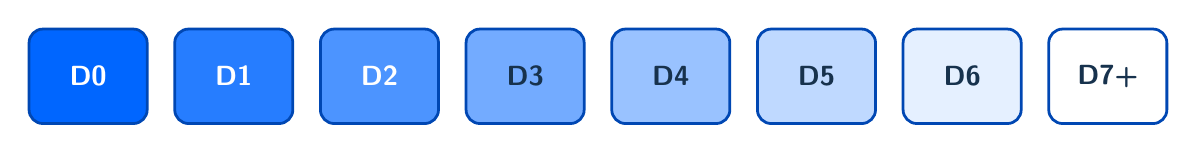
\begin{tikzpicture}[font=\sffamily]
  \node[draw=BARefStroke,fill=BARefDZero,text=white,rounded corners=5pt,line width=1pt,minimum width=15mm,minimum height=12mm] at (0,0) {\textbf{D0}};
  \node[draw=BARefStroke,fill=BARefDOne,text=white,rounded corners=5pt,line width=1pt,minimum width=15mm,minimum height=12mm] at (1.85,0) {\textbf{D1}};
  \node[draw=BARefStroke,fill=BARefDTwo,text=white,rounded corners=5pt,line width=1pt,minimum width=15mm,minimum height=12mm] at (3.70,0) {\textbf{D2}};
  \node[draw=BARefStroke,fill=BARefDThree,text=BARefText,rounded corners=5pt,line width=1pt,minimum width=15mm,minimum height=12mm] at (5.55,0) {\textbf{D3}};
  \node[draw=BARefStroke,fill=BARefDFour,text=BARefText,rounded corners=5pt,line width=1pt,minimum width=15mm,minimum height=12mm] at (7.40,0) {\textbf{D4}};
  \node[draw=BARefStroke,fill=BARefDFive,text=BARefText,rounded corners=5pt,line width=1pt,minimum width=15mm,minimum height=12mm] at (9.25,0) {\textbf{D5}};
  \node[draw=BARefStroke,fill=BARefDSix,text=BARefText,rounded corners=5pt,line width=1pt,minimum width=15mm,minimum height=12mm] at (11.10,0) {\textbf{D6}};
  \node[draw=BARefStroke,fill=BARefDSeven,text=BARefText,rounded corners=5pt,line width=1pt,minimum width=15mm,minimum height=12mm] at (12.95,0) {\textbf{D7+}};
\end{tikzpicture}
\end{center}

\vspace{4mm}
\subsection{Esempio grafico generico di containment}

\begin{center}
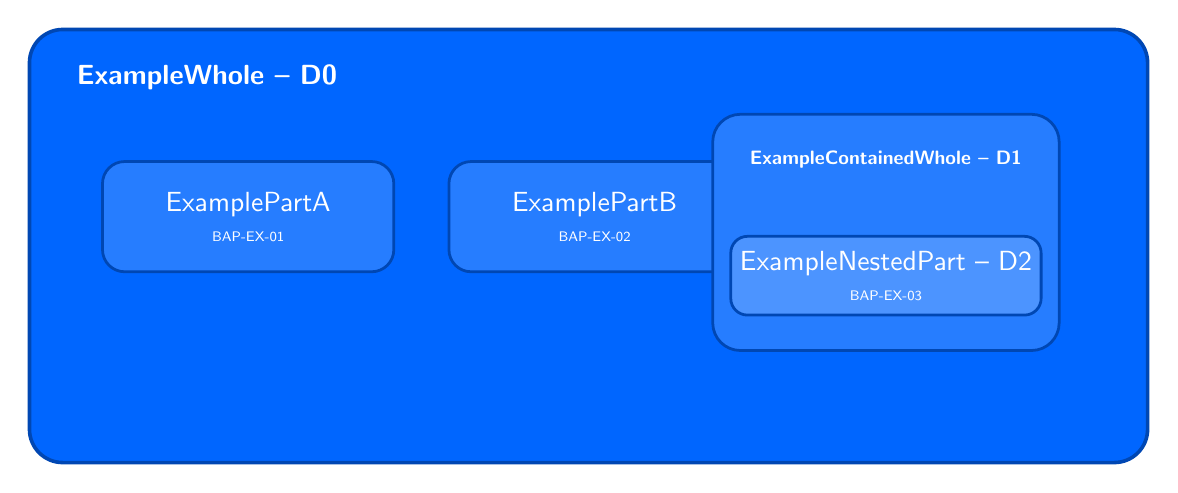
\begin{tikzpicture}[font=\sffamily]
  \node[draw=BARefStroke,fill=BARefDZero,text=white,rounded corners=12pt,
        line width=1.3pt,minimum width=142mm,minimum height=55mm,anchor=north west]
        (outer) at (0,0) {};
  \node[anchor=north west,text=white,font=\sffamily\bfseries] at (0.5,-0.35) {ExampleWhole -- D0};

  \node[draw=BARefStroke,fill=BARefDOne,text=white,rounded corners=8pt,
        line width=1pt,minimum width=37mm,minimum height=14mm,align=center]
        at (2.8,-2.4) {ExamplePartA\\[-0.4mm]{\fontsize{5}{5.4}\selectfont\color{white}BAP-EX-01}};

  \node[draw=BARefStroke,fill=BARefDOne,text=white,rounded corners=8pt,
        line width=1pt,minimum width=37mm,minimum height=14mm,align=center]
        at (7.2,-2.4) {ExamplePartB\\[-0.4mm]{\fontsize{5}{5.4}\selectfont\color{white}BAP-EX-02}};

  \node[draw=BARefStroke,fill=BARefDOne,text=white,rounded corners=10pt,
        line width=1pt,minimum width=44mm,minimum height=30mm,align=center]
        (nested) at (10.9,-2.6) {};
  \node[text=white,font=\sffamily\bfseries\scriptsize,align=center]
        at (10.9,-1.68) {ExampleContainedWhole -- D1};
  \node[draw=BARefStroke,fill=BARefDTwo,text=white,rounded corners=6pt,
        line width=1pt,minimum width=30mm,minimum height=10mm,align=center]
        at (10.9,-3.15) {ExampleNestedPart -- D2\\[-0.4mm]{\fontsize{5}{5.4}\selectfont\color{white}BAP-EX-03}};
\end{tikzpicture}
\end{center}

\begin{ddtaprinciple}[title={HASPART-P03 - containment sostituisce l'edge nella composition view}]
Nella vista di composizione, la presenza della part dentro il frame del whole rappresenta la proposition \texttt{hasPart}; non e' necessario aggiungere anche una freccia \texttt{hasPart}. Gli ID delle proposition possono essere preservati applicando la regola generale \texttt{MERMAID-TRACE-01} alle occurrence interessate.
\end{ddtaprinciple}

\begin{ddtacore}[title={HASPART-P03A - traceability sulla part}]
Quando piu' proposition \texttt{hasPart} descrivono le part dirette dello stesso whole, il trace tag della singola proposition viene collocato \textbf{sotto la label della part corrispondente}. Il whole non ripete tutti gli ID delle relazioni: il containment identifica il whole comune, mentre ogni part conserva il proprio riferimento \BAP{} secondo \texttt{MERMAID-TRACE-01}.
\end{ddtacore}

\subsection{Esempio Mermaid generico}
\begin{lstlisting}
flowchart TB

subgraph ExampleWhole["ExampleWhole"]
  direction TB

  ExamplePartA("ExamplePartA<br/><span style='font-size:7px;color:#FFFFFF'>BAP-EX-01</span>")
  ExamplePartB("ExamplePartB<br/><span style='font-size:7px;color:#FFFFFF'>BAP-EX-02</span>")

  subgraph ExampleContainedWhole["ExampleContainedWhole"]
    ExampleNestedPart("ExampleNestedPart<br/><span style='font-size:7px;color:#FFFFFF'>BAP-EX-03</span>")
  end
end

classDef BAReferentD1 fill:#267DFF,stroke:#0047B3,
  stroke-width:2px,color:#FFFFFF;
classDef BAReferentD2 fill:#4C94FF,stroke:#0047B3,
  stroke-width:2px,color:#FFFFFF;

class ExamplePartA,ExamplePartB BAReferentD1;
class ExampleNestedPart BAReferentD2;

style ExampleWhole fill:#0066FF,stroke:#0047B3,
  stroke-width:2.5px,color:#FFFFFF
style ExampleContainedWhole fill:#267DFF,stroke:#0047B3,
  stroke-width:2.5px,color:#FFFFFF
\end{lstlisting}

\begin{ddtacore}[title={HASPART-P04 - le relazioni esterne puntano al whole}]
Quando un \BAR{} e' espanso a subgraph per mostrare le sue part, una relazione BA che ha quel referent come endpoint deve terminare sul \textbf{frame del whole}, non su una part scelta per convenienza grafica. In Mermaid si usa quindi l'ID del subgraph come source o target dell'edge. Il containment non modifica l'endpoint semantico della proposition esterna.
\end{ddtacore}

\begin{lstlisting}
ExternalActor -->|operator| ExampleWhole
\end{lstlisting}

\begin{ddtaanti}[title={Non dedurre una tassonomia dal livello visuale}]
D0, D1, D2 e i livelli successivi non sono tipi BA. Descrivono soltanto la profondita' della occurrence nella projection corrente. Lo stesso \BAR{} puo' apparire a una profondita' diversa in una view con root differente senza cambiare identita' o semantica.
\end{ddtaanti}
%</MERMAID-ELEMENT:hasPart>

%<MERMAID-ELEMENT:produce>
\clearpage
\section{\texttt{produce}}

\RuleTag\hspace{0.5em}\texttt{semanticOperatorKey = produce}

\subsection{Scopo della rappresentazione}
La proposition \texttt{produce} viene letta graficamente come una funzione che riceve eventuali input, opera attraverso il proprio \texttt{actor} e rende disponibili uno o piu' \texttt{result}. La grafica di \texttt{produce} non assegna lo stile semantico ai result: ogni result conserva o ricevera' la propria regola visuale indipendente.

Esempio generico:

\begin{lstlisting}
BAP-EX-01 - produce
actor  -> ExampleProducer
result -> ExampleResult
\end{lstlisting}

La lettura funzionale e': \texttt{ExampleProducer} produce \texttt{ExampleResult}.

\subsection{Regola grafica candidata}

\begin{tabularx}{\textwidth}{L{39mm}Y}
\toprule
\textbf{Parte BA} & \textbf{Projection Mermaid corrente} \\
\midrule
\texttt{actor} & Black box: rettangolo ad angoli retti, sfondo antracite/nero, bordo nero, testo principale bianco. \\
\texttt{produce} & Freccia direzionale uscente dall'actor con label testuale \texttt{produce} su fondo bianco, bordo sottile e angoli arrotondati. Non viene creato un nodo autonomo \texttt{produce}. \\
\texttt{input} & Quando presente, entra nella black box. La relativa shape dipende dalla regola visuale dell'elemento che occupa il role \texttt{input}. \\
\texttt{result} & Esce dalla black box. La relativa shape e il colore \textbf{non sono definiti da produce}; dipendono dalla regola visuale propria del result. \\
\bottomrule
\end{tabularx}

\begin{ddtacore}[title={PRODUCE-P01 - black box funzionale}]
L'\texttt{actor} di una \texttt{produce} viene proiettato come \textbf{black box rettangolare ad angoli retti}. La black box comunica una funzione/responsabilita' osservata attraverso input e result senza trasformarla graficamente nella sua realizzazione concreta.
\end{ddtacore}

\begin{ddtacore}[title={PRODUCE-P02 - edge label arrotondata}]
La label \texttt{produce} resta associata alla freccia e non diventa un nodo BA. Il target visuale usa \textbf{fondo bianco, bordo sottile e angoli arrotondati} per separare la label dalla linea senza introdurre una nuova shape semantica. Nel renderer Mermaid corrente il trattamento viene applicato alla edge label tramite \texttt{themeCSS}.
\end{ddtacore}

\begin{lstlisting}
%%{init: {
  "theme": "base",
  "themeCSS": ".edgeLabel p { background:#FFFFFF !important; border:1px solid #B8CBE8 !important; border-radius:10px !important; padding:2px 7px !important; }"
}}%%
\end{lstlisting}

\subsection{Classe visuale dell'actor}
La classe e' nominata per il significato di projection, non per il colore:

\begin{lstlisting}
classDef BAProduceActor \
    fill:#212121, \
    stroke:#000000, \
    stroke-width:2px, \
    color:#FFFFFF;
\end{lstlisting}

La sintassi rettangolare Mermaid \texttt{["..."]} mantiene gli angoli retti; non vengono aggiunti \texttt{rx}/\texttt{ry}. Nella projection \texttt{produce}, l'actor e' anche l'anchor della proposition: il relativo ID \BAP{} viene quindi riportato sotto il nome dell'actor secondo \texttt{MERMAID-TRACE-01}.

\subsection{Esempio Mermaid minimo}
Il result \texttt{ExampleResult} e' lasciato intenzionalmente al solo fallback della baseline: la sua forma canonica dipende dalla regola visuale dell'elemento/famiglia che occupa il role \texttt{result} e \textbf{non} dalla regola \texttt{produce}.

Applicare prima la baseline \texttt{MERMAID-BASE-01}; il blocco specifico della \texttt{produce} resta quindi compatto:

\begin{lstlisting}
flowchart LR

ExampleProducer["ExampleProducer<br/><span style='font-size:7px;color:#FFFFFF'>BAP-EX-01</span>"]
ExampleResult["ExampleResult"]

ExampleProducer -->|produce| ExampleResult

classDef BAProduceActor \
  fill:#212121,stroke:#000000,stroke-width:2px,color:#FFFFFF;
class ExampleProducer BAProduceActor;
\end{lstlisting}


\subsection{Esempio grafico visivo}
La figura seguente mostra il \textbf{target visuale corrente} della sola regola \texttt{produce}. Il nodo di destra usa volutamente il fallback della baseline: non assegna al result una forma derivata da \texttt{produce}. Il disegno in guida e' un riferimento visuale della convenzione; il sorgente Mermaid resta la forma eseguibile da verificare nel renderer scelto.

\vspace{3mm}
\begin{center}
\begin{tikzpicture}[>=Latex,font=\sffamily]
  \node[
    draw=black,
    fill=BAProduceFill,
    text=white,
    line width=1.1pt,
    minimum width=54mm,
    minimum height=16mm,
    align=center,
    inner sep=3mm
  ] (actor) {\textbf{ExampleProducer}\\[-0.2mm]
             {\fontsize{5.5}{6}\selectfont\color{white}BAP-EX-01}};

  \node[
    draw=DDTAGray,
    fill=white,
    text=DDTANavy,
    line width=0.8pt,
    minimum width=48mm,
    minimum height=14mm,
    align=center,
    inner sep=3mm,
    right=36mm of actor
  ] (result) {ExampleResult};

  \draw[-{Latex[length=3mm,width=2mm]},line width=1.1pt,color=DDTAGray]
    (actor.east) -- node[midway,above=2pt,fill=white,draw=DDTABlue,line width=0.35pt,rounded corners=4pt,inner xsep=5pt,inner ysep=2pt,text=DDTANavy]{\small\texttt{produce}} (result.west);
\end{tikzpicture}
\end{center}
\vspace{2mm}

\begin{ddtaprinciple}[title={Che cosa e' fissato dalla figura}]
La figura fissa soltanto gli aspetti specifici di \texttt{produce}: \textbf{black box ad angoli retti} per l'\texttt{actor} e freccia uscente con label \texttt{produce} su pill bianca arrotondata con bordo sottile. Il trace tag applica la regola generale \texttt{MERMAID-TRACE-01}. Forma e stile del result restano intenzionalmente fuori da questa pagina.
\end{ddtaprinciple}

\begin{ddtaanti}[title={Non inferire lo stile del result da produce}]
Il fatto che un elemento occupi il role \texttt{result} non autorizza a renderlo con la stessa black box, con una shape ``output'' generica o con un colore scelto da \texttt{produce}. \texttt{produce} governa il pattern di connessione; lo stile del result appartiene alla regola visuale dell'elemento che occupa quel role.
\end{ddtaanti}
%</MERMAID-ELEMENT:produce>


%<MERMAID-ELEMENT:dependOn>
\clearpage
\section{\texttt{dependOn}}

\RuleTag\hspace{0.5em}\texttt{semanticOperatorKey = dependOn}

\subsection{Scopo della rappresentazione}
La proposition \texttt{dependOn} esprime una dipendenza direzionale fra un \texttt{dependent} e un \texttt{prerequisite}. La projection deve rendere leggibile la dipendenza senza attribuire ai due referent un nuovo semantic kind e senza competere visivamente con relazioni funzionali piu' strutturanti.

Esempio generico:

\begin{lstlisting}
BAP-EX-02 - dependOn
dependent    -> ExampleDependent
prerequisite -> ExamplePrerequisite
\end{lstlisting}

La lettura grafica e': \texttt{ExampleDependent} dipende da \texttt{ExamplePrerequisite}.

\subsection{Regola grafica candidata}

\begin{tabularx}{\textwidth}{L{39mm}Y}
\toprule
\textbf{Parte BA} & \textbf{Projection Mermaid corrente} \\
\midrule
\texttt{dependent} & Sorgente della freccia. Mantiene la shape e lo stile propri del referent. E' l'anchor del trace tag della proposition. \\
\texttt{dependOn} & Freccia direzionale tratteggiata, sottile, in famiglia giallo/ocra. La label e' una pill arrotondata con fondo giallo chiaro, bordo ocra e testo ocra scuro. \\
\texttt{prerequisite} & Destinazione della freccia. Mantiene la shape e lo stile propri del referent. Se e' visualizzato come whole/subgraph, la relazione termina sul whole nel suo complesso. \\
\bottomrule
\end{tabularx}

\begin{ddtacore}[title={DEPENDON-P01 - direzione dependent verso prerequisite}]
La direzione della freccia segue direttamente i role BA: \texttt{dependent} $\rightarrow$ \texttt{prerequisite}. La label \texttt{dependOn} resta associata all'edge e non diventa un nodo BA autonomo.
\end{ddtacore}

\begin{ddtacore}[title={DEPENDON-P02 - peso visuale secondario}]
La relazione usa stroke \texttt{\#C69214}, spessore \texttt{1.5px} e tratteggio \texttt{6 4}. Il trattamento leggero rende la dipendenza informativa distinguibile senza farla dominare sulla struttura funzionale o di containment della stessa view.
\end{ddtacore}

\begin{ddtacore}[title={DEPENDON-P03 - edge label giallo/ocra arrotondata}]
La label \texttt{dependOn} usa fondo \texttt{\#FFF4CC}, bordo \texttt{\#C69214}, testo \texttt{\#7A5A00} e angoli arrotondati. La pill resta una label dell'edge: il trattamento grafico non introduce un nuovo referent.
\end{ddtacore}

\subsection{Traceability della proposition}
Nella projection \texttt{dependOn}, il \texttt{dependent} e' l'anchor della proposition. Il relativo ID \BAP{} viene quindi riportato sotto la label del dependent, in piccolo e in bianco, secondo \texttt{MERMAID-TRACE-01}. Il prerequisite non ripete lo stesso ID.

\subsection{Esempio Mermaid minimo}
L'esempio seguente isola la sola relazione \texttt{dependOn}; poiche' contiene una sola edge label, il \texttt{themeCSS} puo' applicare direttamente il trattamento giallo/ocra alla label senza influenzare altri operatori.

\begin{lstlisting}
%%{init: {
  "theme": "base",
  "themeCSS": ".edgeLabel p { background:#FFF4CC !important; border:1px solid #C69214 !important; border-radius:10px !important; padding:2px 7px !important; color:#7A5A00 !important; }"
}}%%

flowchart LR

ExampleDependent("ExampleDependent<br/><span style='font-size:7px;color:#FFFFFF'>BAP-EX-02</span>")
ExamplePrerequisite("ExamplePrerequisite")

ExampleDependent -.->|dependOn| ExamplePrerequisite

classDef BAReferentD0 fill:#0066FF,stroke:#0047B3,
  stroke-width:2px,color:#FFFFFF;
class ExampleDependent,ExamplePrerequisite BAReferentD0;

linkStyle 0 stroke:#C69214,stroke-width:1.5px,
  stroke-dasharray:6 4;
\end{lstlisting}

\begin{ddtaworking}[title={Coesistenza di edge label con stili diversi}]
In una view composita possono coesistere operatori con edge label differenti, per esempio \texttt{produce} e \texttt{dependOn}. La regola semantica fissa il target visuale di ciascun operatore; l'eventuale selettore CSS necessario a stilizzare una singola edge label deve essere verificato nel renderer adottato e non deve alterare le label degli altri operatori.
\end{ddtaworking}

\subsection{Esempio grafico visivo}
\begin{center}
\begin{tikzpicture}[>=Latex,font=\sffamily]
  \node[
    draw=BARefStroke,fill=BARefDZero,text=white,
    rounded corners=6pt,line width=1pt,
    minimum width=48mm,minimum height=15mm,align=center
  ] (dep) {\textbf{ExampleDependent}\\[-0.3mm]
           {\fontsize{5.5}{6}\selectfont\color{white}BAP-EX-02}};

  \node[
    draw=BARefStroke,fill=BARefDZero,text=white,
    rounded corners=6pt,line width=1pt,
    minimum width=48mm,minimum height=15mm,align=center,
    right=48mm of dep
  ] (pre) {\textbf{ExamplePrerequisite}};

  \draw[-{Latex[length=2.6mm,width=1.8mm]},
        draw=BADependStroke,line width=0.65pt,dash pattern=on 3.2pt off 2.1pt]
    (dep.east) --
    node[midway,above=2pt,fill=BADependFill,draw=BADependStroke,
         line width=0.45pt,rounded corners=4pt,
         inner xsep=5pt,inner ysep=2pt,text=BADependText]
         {\small\texttt{dependOn}}
    (pre.west);
\end{tikzpicture}
\end{center}

\begin{ddtaprinciple}[title={DEPENDON-P04 - il prerequisite conserva la propria topology}]
Se il prerequisite e' un \BAR{} espanso a subgraph perche' nella stessa view sono mostrate le sue part, la freccia \texttt{dependOn} termina sul frame del whole. Non viene scelta arbitrariamente una part interna come destinazione. Il giallo/ocra appartiene soltanto all'edge e alla label: i referent collegati mantengono shape, fill, depth palette e identita' determinati dalle rispettive regole visuali.
\end{ddtaprinciple}

%</MERMAID-ELEMENT:dependOn>



%<MERMAID-ELEMENT:realize>
\clearpage
\section{\texttt{realize}}

\RuleTag\hspace{0.5em}\texttt{semanticOperatorKey = realize}

\subsection{Scopo della rappresentazione}
La proposition \texttt{realize} collega una responsabilita' o funzione astratta alla realizzazione concreta che la attua nella baseline osservata. La projection deve mantenere distinte le due identita': l'\texttt{abstract} conserva la propria famiglia visuale, mentre la \texttt{realization} viene resa riconoscibile mediante una famiglia grigia dedicata alla relation view.

Esempio generico:

\begin{lstlisting}
BAP-EX-03 - realize
abstract    -> ExampleAbstract
realization -> ExampleRealization
\end{lstlisting}

La lettura grafica e': \texttt{ExampleRealization} realizza \texttt{ExampleAbstract}.

\begin{ddtacore}[title={REALIZE-P01 - direzione realization verso abstract}]
La freccia segue direttamente i role BA: \texttt{realization} $\rightarrow$ \texttt{abstract}. L'edge usa stroke grigio \texttt{\#5F6368}, spessore \texttt{1.8px} e tratteggio \texttt{6 4}. La label \texttt{realize} resta associata all'edge e non diventa un nodo BA autonomo.
\end{ddtacore}

\begin{ddtacore}[title={REALIZE-P02 - famiglia grigia della realization}]
L'occurrence che occupa il role \texttt{realization} usa come livello D0 il fill \texttt{\#5F6368}. Quando la realization e' espansa per mostrare le proprie part, il whole viene proiettato come subgraph/frame con stroke \texttt{\#3F4347}, spessore \texttt{2.5px} e bordo tratteggiato \texttt{6 4}. Il tratteggio del frame identifica la topology di realization nella projection; non introduce un nuovo semantic kind BA.
\end{ddtacore}

\begin{ddtacore}[title={REALIZE-P03 - depth palette interna alla realization}]
Se nella stessa view sono mostrate proposition \texttt{hasPart} del referent che occupa il role \texttt{realization}, le part contenute usano la stessa famiglia grigia e vengono schiarite di \textbf{15 punti percentuali verso il bianco per ogni livello di containment}. Le part hanno bordo continuo; il bordo tratteggiato resta sul whole che costituisce l'endpoint della proposition \texttt{realize}.
\end{ddtacore}

\begin{ddtaprinciple}[title={L'abstract conserva il proprio stile}]
\texttt{realize} non riclassifica l'\texttt{abstract}. Shape, fill e topology dell'abstract restano determinati dalle altre proposition e dalle altre regole visuali applicabili nella view. La famiglia grigia appartiene alla projection della realization e al suo containment interno.
\end{ddtaprinciple}

\subsection{Traceability}
L'anchor della proposition \texttt{realize} e' la \texttt{realization}: l'ID della \BAP{} viene riportato sotto la label del nodo o del subgraph che rappresenta la realization secondo \texttt{MERMAID-TRACE-01}. Le proposition \texttt{hasPart} interne mantengono invece il proprio trace tag sotto la part corrispondente, secondo \texttt{HASPART-P03A}.

\subsection{Esempio Mermaid generico}
\begin{lstlisting}
%%{init: {
  "theme": "base",
  "themeCSS": ".cluster rect { rx:28px !important; ry:28px !important; }"
}}%%

flowchart LR

ExampleAbstract("ExampleAbstract")

subgraph ExampleRealization["ExampleRealization<br/><span style='font-size:7px;color:#FFFFFF'>BAP-EX-03</span>"]
  direction TB
  ExampleStageA("ExampleStageA<br/><span style='font-size:7px;color:#FFFFFF'>BAP-EX-04</span>")
  ExampleStageB("ExampleStageB<br/><span style='font-size:7px;color:#FFFFFF'>BAP-EX-05</span>")
end

ExampleRealization -.->|realize| ExampleAbstract

classDef BAReferentD0 fill:#0066FF,stroke:#0047B3,
  stroke-width:2px,color:#FFFFFF;
classDef BARealizationD1 fill:#777A7F,stroke:#3F4347,
  stroke-width:2px,color:#FFFFFF;

class ExampleAbstract BAReferentD0;
class ExampleStageA,ExampleStageB BARealizationD1;

style ExampleRealization fill:#5F6368,stroke:#3F4347,
  stroke-width:2.5px,stroke-dasharray:6 4,color:#FFFFFF

linkStyle 0 stroke:#5F6368,stroke-width:1.8px,
  stroke-dasharray:6 4;
\end{lstlisting}

\subsection{Esempio grafico visivo}
\begin{center}
\begin{tikzpicture}[>=Latex,font=\sffamily]
  \node[
    draw=BARefStroke,fill=BARefDZero,text=white,
    rounded corners=6pt,line width=1pt,
    minimum width=47mm,minimum height=15mm,align=center
  ] (abstract) at (10.7,0) {\textbf{ExampleAbstract}};

  \node[
    draw=BARealizeStroke,fill=BARealizeDZero,text=white,
    rounded corners=11pt,line width=1.2pt,
    dash pattern=on 3.2pt off 2.1pt,
    minimum width=68mm,minimum height=42mm,align=center
  ] (realframe) at (4.0,0) {};

  \node[text=white,font=\sffamily\bfseries\scriptsize,align=center]
    at (4.0,1.38) {ExampleRealization\\[-0.5mm]
    {\fontsize{5.2}{5.6}\selectfont\color{white}BAP-EX-03}};

  \node[
    draw=BARealizeStroke,fill=BARealizeDOne,text=white,
    rounded corners=6pt,line width=0.9pt,
    minimum width=26mm,minimum height=10mm,align=center
  ] at (2.45,-0.65) {ExampleStageA};

  \node[
    draw=BARealizeStroke,fill=BARealizeDOne,text=white,
    rounded corners=6pt,line width=0.9pt,
    minimum width=26mm,minimum height=10mm,align=center
  ] at (5.55,-0.65) {ExampleStageB};

  \draw[-{Latex[length=2.6mm,width=1.8mm]},
        draw=BARealizeDZero,line width=0.8pt,
        dash pattern=on 3.2pt off 2.1pt]
    (realframe.east) --
    node[midway,above=2pt,fill=white,draw=BARealizeDZero,
         line width=0.4pt,rounded corners=4pt,
         inner xsep=5pt,inner ysep=2pt,text=BARealizeStroke]
         {\small\texttt{realize}}
    (abstract.west);
\end{tikzpicture}
\end{center}

\begin{ddtaanti}[title={Non propagare il tratteggio alle part}]
Il bordo tratteggiato non significa ``componente tecnico'' e non viene ereditato automaticamente dalle part. Le part interne mantengono bordo continuo e ricevono soltanto la schiaritura di depth della famiglia grigia, salvo che una proposition indipendente richieda per esse un'altra projection.
\end{ddtaanti}


\clearpage
\section*{Scala cromatica completa della famiglia \texttt{realize}}

La palette della realization applica la stessa regola deterministica di schiaritura usata per il containment: a partire dal base fill \texttt{\#5F6368}, il livello \(D_d\) e' ottenuto miscelando il colore base verso il bianco di \(L(d)=\min(15d,100)\%\). La scala e' una proprieta' grafica della projection e non una tassonomia BA.

\begin{center}
\begin{tabular}{c c c c}
\toprule
\textbf{Depth} & \textbf{Schiaritura} & \textbf{Fill} & \textbf{Testo principale} \\
\midrule
D0 & 0\%   & \texttt{\#5F6368} & \texttt{\#FFFFFF} \\
D1 & 15\%  & \texttt{\#777A7F} & \texttt{\#FFFFFF} \\
D2 & 30\%  & \texttt{\#8F9295} & \texttt{\#17324D} \\
D3 & 45\%  & \texttt{\#A7A9AC} & \texttt{\#17324D} \\
D4 & 60\%  & \texttt{\#BFC1C3} & \texttt{\#17324D} \\
D5 & 75\%  & \texttt{\#D7D8D9} & \texttt{\#17324D} \\
D6 & 90\%  & \texttt{\#EFEFF0} & \texttt{\#17324D} \\
D7+ & 100\% & \texttt{\#FFFFFF} & \texttt{\#17324D} \\
\bottomrule
\end{tabular}
\end{center}

\vspace{2mm}
\begin{center}
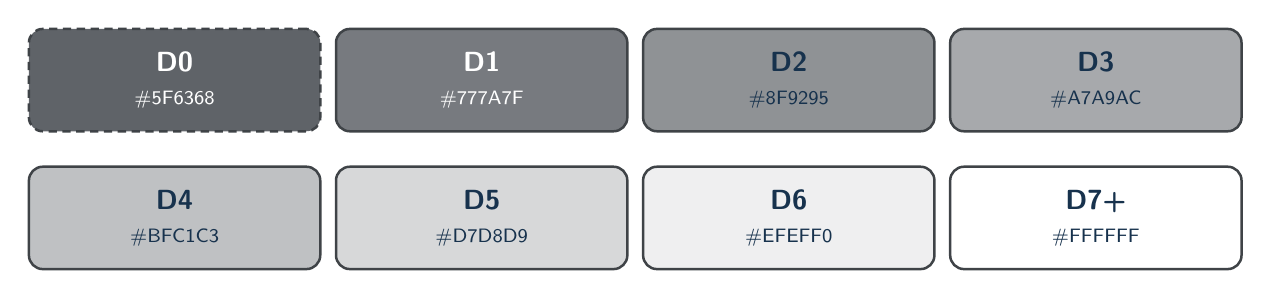
\begin{tikzpicture}[font=\sffamily]
  \node[draw=BARealizeStroke,fill=BARealizeDZero,text=white,rounded corners=5pt,line width=0.9pt,dash pattern=on 3pt off 2pt,minimum width=37mm,minimum height=13mm,align=center] at (2.2,0) {\textbf{D0}\\{\scriptsize \#5F6368}};
  \node[draw=BARealizeStroke,fill=BARealizeDOne,text=white,rounded corners=5pt,line width=0.9pt,minimum width=37mm,minimum height=13mm,align=center] at (6.1,0) {\textbf{D1}\\{\scriptsize \#777A7F}};
  \node[draw=BARealizeStroke,fill=BARealizeDTwo,text=BARefText,rounded corners=5pt,line width=0.9pt,minimum width=37mm,minimum height=13mm,align=center] at (10.0,0) {\textbf{D2}\\{\scriptsize \#8F9295}};
  \node[draw=BARealizeStroke,fill=BARealizeDThree,text=BARefText,rounded corners=5pt,line width=0.9pt,minimum width=37mm,minimum height=13mm,align=center] at (13.9,0) {\textbf{D3}\\{\scriptsize \#A7A9AC}};

  \node[draw=BARealizeStroke,fill=BARealizeDFour,text=BARefText,rounded corners=5pt,line width=0.9pt,minimum width=37mm,minimum height=13mm,align=center] at (2.2,-1.75) {\textbf{D4}\\{\scriptsize \#BFC1C3}};
  \node[draw=BARealizeStroke,fill=BARealizeDFive,text=BARefText,rounded corners=5pt,line width=0.9pt,minimum width=37mm,minimum height=13mm,align=center] at (6.1,-1.75) {\textbf{D5}\\{\scriptsize \#D7D8D9}};
  \node[draw=BARealizeStroke,fill=BARealizeDSix,text=BARefText,rounded corners=5pt,line width=0.9pt,minimum width=37mm,minimum height=13mm,align=center] at (10.0,-1.75) {\textbf{D6}\\{\scriptsize \#EFEFF0}};
  \node[draw=BARealizeStroke,fill=BARealizeDSeven,text=BARefText,rounded corners=5pt,line width=0.9pt,minimum width=37mm,minimum height=13mm,align=center] at (13.9,-1.75) {\textbf{D7+}\\{\scriptsize \#FFFFFF}};
\end{tikzpicture}
\end{center}

\begin{ddtacore}[title={REALIZE-P04 - valori espliciti nel sorgente Mermaid}]
Per ridurre differenze fra renderer, i valori D0--D7 vengono fissati esplicitamente nel sorgente. D0 e' il whole della realization; D1--D7 sono disponibili per le part annidate in base alla depth effettivamente mostrata nella view.
\end{ddtacore}

\clearpage
\subsection*{Mermaid palette test completo}
Il blocco seguente rende disponibili tutti i livelli della famiglia \texttt{realize} per test di renderer e per view con containment profondo. Il file di prova standalone usa gli stessi valori.

\begin{lstlisting}
classDef BARealizationD0 fill:#5F6368,stroke:#3F4347,
  stroke-width:2.5px,color:#FFFFFF;
classDef BARealizationD1 fill:#777A7F,stroke:#3F4347,
  stroke-width:2px,color:#FFFFFF;
classDef BARealizationD2 fill:#8F9295,stroke:#3F4347,
  stroke-width:2px,color:#17324D;
classDef BARealizationD3 fill:#A7A9AC,stroke:#3F4347,
  stroke-width:2px,color:#17324D;
classDef BARealizationD4 fill:#BFC1C3,stroke:#3F4347,
  stroke-width:2px,color:#17324D;
classDef BARealizationD5 fill:#D7D8D9,stroke:#3F4347,
  stroke-width:2px,color:#17324D;
classDef BARealizationD6 fill:#EFEFF0,stroke:#3F4347,
  stroke-width:2px,color:#17324D;
classDef BARealizationD7 fill:#FFFFFF,stroke:#3F4347,
  stroke-width:2px,color:#17324D;
\end{lstlisting}

\begin{ddtaprinciple}[title={Il trace tag resta bianco}]
Come stabilito da \texttt{MERMAID-TRACE-01}, il trace tag \BAP{} resta sempre bianco anche ai livelli chiari. Il cambio di colore indicato nella tabella riguarda il testo principale del nodo; la traceability autorevole resta nel sorgente anche quando il tag e' poco visibile.
\end{ddtaprinciple}

%</MERMAID-ELEMENT:realize>

\end{document}

